\chapter{Using Nexys4 boards as a MEGA65}

\section{Building your own MEGA65 Compatible Computer}

You can build your own MEGA65-compatible computer by using either a Nexys4DDR (aka. Nexys A7) or the older Nexys4 (Non-DDR) FPGA development boards.
This appendix describes the process to set up a Nexys4DDR (Nexys A7) board for this purpose (which is the newer, preferred board).
The older non-DDR Nexys4 board is also supported, and the instructions are the same, except that
you must use a bitstream designed for that board.
Using a Nexys4DDR bitstream on a non-DDR Nexys4 board, or vice versa, may cause irreparable damage to your board, so make sure
you have the correct bitstream to suit your board.


DISCLAIMER: M.E.G.A cannot take any responsibility for any damage that may occur to your Nexys4DDR/NexysA7/Nexys4 boards.

\newpage

\section{Working Nexys4 Boards}

There are currently 3 Nexys FPGA boards which can be setup as a MEGA65:

\begin{minipage}{\linewidth}
  \subsection{The Nexys4 board}

  No longer manufactured but still available for sale on some websites with old stock.

  \begin{center}
    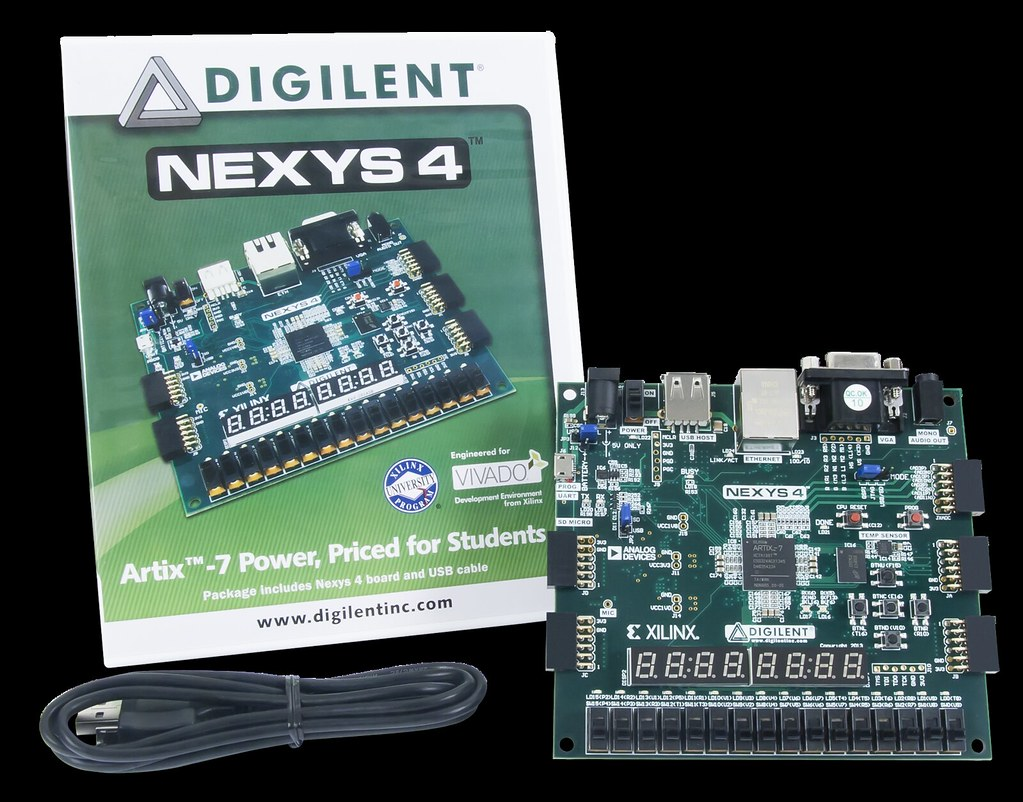
\includegraphics[width=0.4\linewidth]{images/img001_nexys4_board.jpg}
  \end{center}

  Documentation:

  \begin{itemize}
    \item \url{https://reference.digilentinc.com/reference/programmable-logic/nexys-4/reference-manual}
    \item \url{https://reference.digilentinc.com/\_media/reference/programmable-logic/nexys-4/nexys4\_rm.pdf}
  \end{itemize}
\end{minipage}

\begin{minipage}{\linewidth}
  \subsection{The Nexys4DDR board}

  No longer manufactured but still available for sale on some websites with old stock.

  \begin{center}
    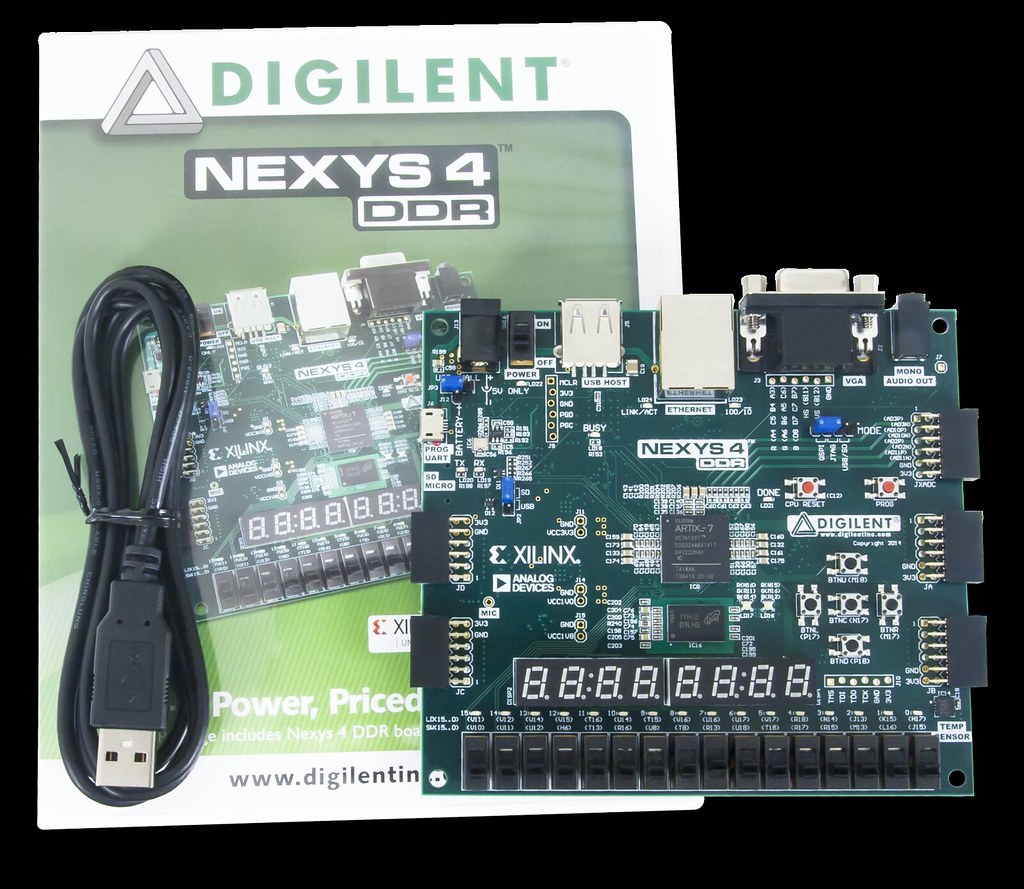
\includegraphics[width=0.4\linewidth]{images/img002_nexys4_ddr_board.jpg}
  \end{center}

  Documentation:

  \begin{itemize}
    \item \url{https://reference.digilentinc.com/reference/programmable-logic/nexys-4-ddr/reference-manual}
    \item \url{https://reference.digilentinc.com/\_media/reference/programmable-logic/nexys-4-ddr/nexys4ddr\_rm.pdf}
  \end{itemize}
\end{minipage}

\begin{minipage}{\linewidth}
  \subsection{The Nexys A7}

  This is the re-branded version of the above Nexys4 DDR board:

  \begin{center}
    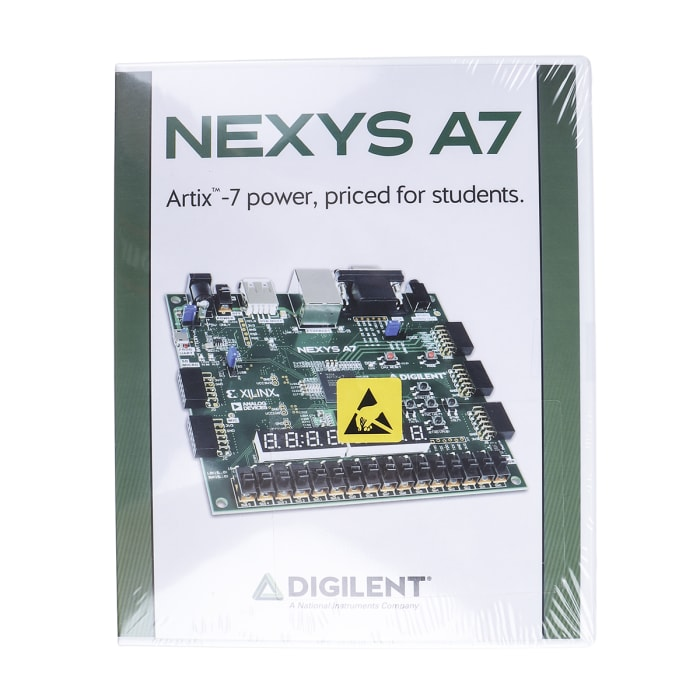
\includegraphics[width=0.4\linewidth]{images/img003_nexysA7_board.jpg}
  \end{center}

  Documentation:

  \begin{itemize}
    \item \url{https://reference.digilentinc.com/reference/programmable-logic/nexys-a7/reference-manual}
    \item \url{https://reference.digilentinc.com/\_media/reference/programmable-logic/nexys-a7/nexys-a7\_rm.pdf}
  \end{itemize}
\end{minipage}

\newpage

\section{Power, Jumpers, Switches and Buttons}

This top-down picture highlights the key jumper positions of interest on the Nexys4 board:

  \begin{center}
    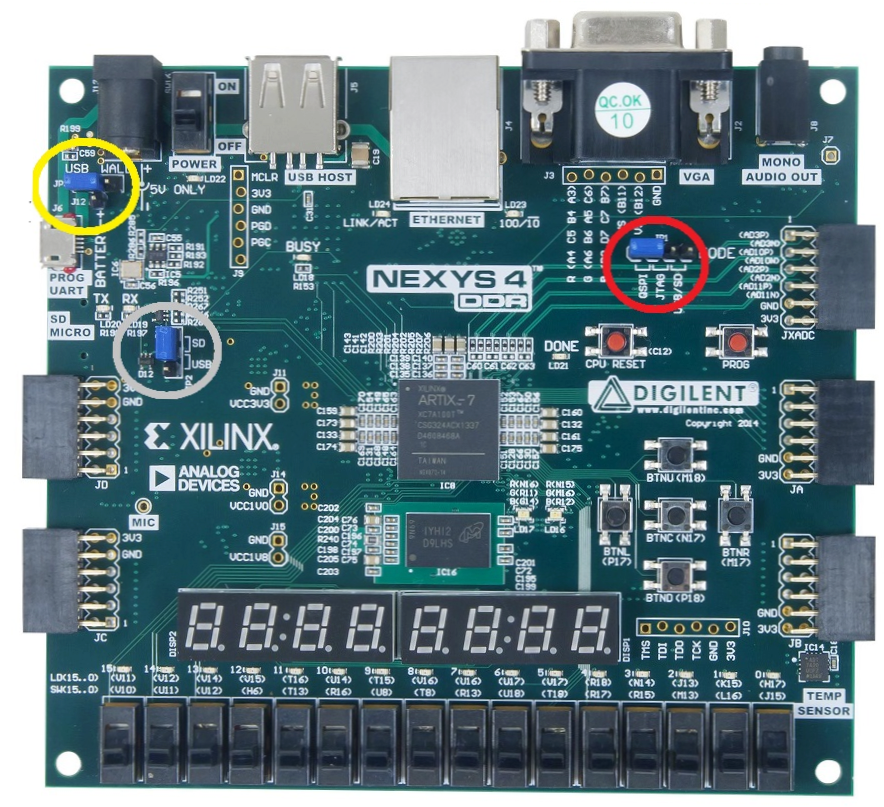
\includegraphics[width=0.9\linewidth]{images/nexys4_jumpers.png}
  \end{center}

The Nexys4 boards can be powered in two ways: using an external power supply, or from a standard USB port.

\subsection{Micro-USB Power}

\includegraphics[width=5cm]{images/illustrations/nexys-micro-usb-power.pdf}

Connect your micro-usb cable to a USB port on a USB charger or PC to provide power. Connect the other end to the Nexys4's micro-usb connector. Place the JP3 jumper on pins 1 and 2 to select USB power. Use the switch to turn on the Nexys4.

\subsection{External Power Supply}

\hspace*{1.7cm}
\includegraphics[width=3.2cm]{images/illustrations/nexys-power-supply.pdf}

The MEGA65 core can consume a lot of power, and a standard USB port could potentionally be too little for the Nexys4 board. In particular, writing to the SD card might hang or perform odd behaviour. Therefore you should consider a 5V power supply.

Digilent sell a power supply for the Nexys4 board, and we recommend you use this to ensure you avoid the risk of damage to your Nexys4 board. The chosen power supply should be center positive, 2.1mm internal diameter plug, and should deliver 4.5VDC to 5.5VDC rated at least 1 Amp.

Connect the power supply cable to the supply plug of the Nexys4. Place the JP3 jumper on pins 2 and 3 to select WALL power. Use the switch to turn on the Nexys4.

\subsection{Other Jumpers and Switches}

For your initial set up, we'd suggest you set the following jumpers on your Nexys4 board to these positions:

\begin{itemize}
  \item{JP1} - USB/SD
  \item{JP2} - SD
\end{itemize}

This will assure that the bitstream files will get loaded from your sd-card on start-up.

At some later stage, you may prefer to load the bitstream from the on-board QSPI flash, and at that point, you can revisit your JP1 jumper setting and adjust it to the QSPI position.

% XXX - Image of board highlighting the jumpers

All 16 switches on the lower edge of the board must be set to the off position.


\subsection{Connections and Peripherals}

\includegraphics[width=\linewidth]{images/illustrations/nexys-connectors.pdf}

A USB keyboard can be connected to the USB port. Only a keyboard that lacks a USB hub will work with the Nexys4 board.  Generally, extremely cheap keyboards will work, while more expensive keyboards tend to have a USB hub integrated, and will not work.  You may need to try several keyboards before you find one that works.

You can connect a VGA monitor to the VGA port.

The mono audio-out jack can be connected to the line-in of an amplifier.


\subsection{Communicating with your PC}

There may be occasions where you wish to communicate with your Nexys4 board from your PC, in order to perform activities such as:

\begin{itemize}
  \item Flash your QSPI flash chip via Vivado
  \item Upload bitstream files directly from your PC (via m65 tool)
  \item Make use of support tools such as M65Connect, m65, mega65\_ftp, m65dbg, etc
\end{itemize}

On such occasions, you will need to connect your micro-usb cable up to your PC.

\includegraphics[width=5cm]{images/illustrations/nexys-micro-usb-power.pdf}

\subsection{Onboard buttons}

\begin{center}
  \includegraphics[width=3.2cm]{images/illustrations/nexys-reset-buttons.pdf}
\end{center}

The ``CPU RESET'' button will reset the MEGA65 when pressed, while the ``PROG'' button will cause the FPGA itself to reload the MEGA65
core.  The main difference between the two is that CPU RESET is faster, and does not clear the contents of memory, while the FPGA button
is slower, and does reset the contents of memory.

\begin{center}
  \includegraphics[width=3.2cm]{images/illustrations/nexys-five-buttons.pdf}
\end{center}

Two of the five buttons in the cross arrangement can also be used:  BTND acts as though you have pressed the \megakey{RESTORE} key, while BTNC will trigger an IRQ, as though the IRQ line had been pulled to ground.

\section{Keyboard}

The keyboard layout is positional rather than logical.
This means that keys in similar positions to the keys on a C65 keyboard will have similar function.
This relationship assumes that your USB keyboard uses a US keyboard layout.

To help you locate what the various MEGA65 keys are mapped to, the MEGA65 has a built-in virtual keyboard test feature. This can be accessed in two ways.

The easiest way is to keep the \specialkey{ALT} key held in while turning on the Nexys4, or resetting the Nexys4 with the ``PROG'' button. The configure menu will be presented and by pressing 3, the virtual keyboard will be presented on a black background.

\includegraphics[width=\linewidth]{images/illustrations/virtual-keyboard.pdf}

Pressing a key on the USB keyboard will show the highlighted key on the virtual keyboard to help you identify the key mapping.

The other way to access the virtual keyboard is from within the MEGA65. Hold \megasymbolkey and press \megakey{TAB} to access the Matrix Mode Debugger. From here, enter the following:

\screentextwide{s ffd3615 ff}

This will open a semi-transparent virtual keyboard at the top of the screen. Alternatively:

\screentextwide{s ffd3615 ff ff}

This will open a semi-transparent virtual keyboard in the centre of the screen.

Hold \megasymbolkey and press \megakey{TAB} to exit Matrix Mode Debugger and return to the MEGA65.

\subsection{Some key mappings with a USB keyboard}

The \megakey{RESTORE} key is mapped to the PAGE UP key.

The \specialkey{RUN STOP}  key is mapped to the ESC key.

\newpage

\section{Preparing microSDHC card}

The MEGA65 requires an SDHC card of between 4GB and 64GB capacity.  Some SDXC cards may work, however, this is not officially supported.

Preparation steps for the Nexys4 board's sd-card share much in common with the steps needed for real MEGA65 hardware, and as such, it is worth having a look over the \nameref{cha:configuring} chapter if you ever need details. 

So in this section, we'll provide more details on the distinctive steps, and be more brief on the common steps.

One point of distinction between the Nexys board and the real MEGA65 hardware is that the latter already has a default bitstream/core provided, which permits you to format your sd-card in the specific style required by the MEGA65.

For Nexys board owners however, you have no such default bitstream, so will need to prepare one on your sd-card via the steps below.

\subsection{Bitstream File}

Visit the following url:

\url{https://mega.scryptos.com/sharefolder-link/MEGA/MEGA65+filehost/Bitstreams/Jenkins-Out/mega65-core/development/}

Sort the list of build folders by 'Date' and click on the latest:

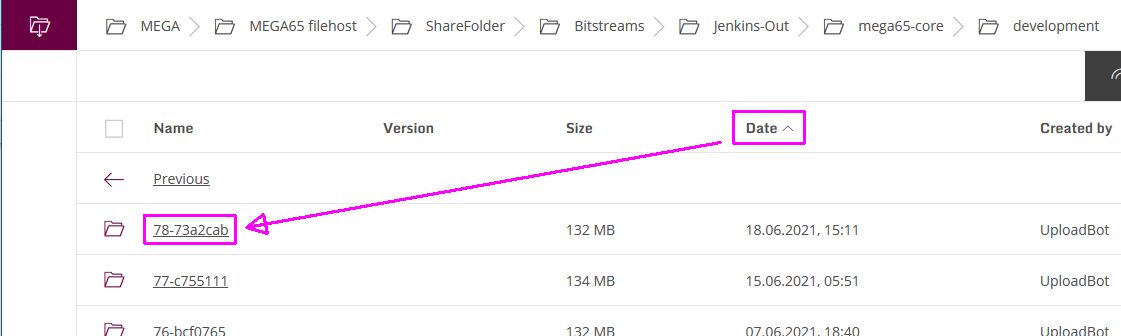
\includegraphics[width=\linewidth]{images/latest_bitstream.png}

Download either:

\begin{itemize}
  \item{\textbf{nexys4.bit} (for Nexys4 PSRAM boards)}
  \item{\textbf{nexys4dd4-widget.bit} (for Nexys4 DDR boards)}
  \item{You can also find bitstream files for various other m65 targets here (mega65r2, mega65r3)}
  \item{You can also find core (.cor) files located here (See \nameref{cha:cores} chapter for more details on how to make use of them)}
\end{itemize}


\subsection{Preparation Steps}

The steps are:

\begin{itemize}
  \item{Format the SD card} in a convenient computer using the FAT32 file-system.  The MEGA65 and Nexys4 boards do not understand other
file systems, especially the exFAT file system.
\item{Copy} your bitstream file (with name ending in ``.bit'') onto the SD card.
\item{Insert} the SD card into the SD card slot on the under-side of the Nexys4 board.
\item{Turn on} the Nexys4 board.
\item{Enter the Utility Menu} by holding the \megakey{ALT} key down on the USB keyboard you have connected to the Nexys4 board.
\item{Enter the FDISK/FORMAT tool} by pressing 2 when the option appears on the MEGA65 boot screen.
\item{Follow the prompts} in the FDISK/FORMAT program to again format the SD card for use by the MEGA65. \\
  \\
  The FDISK tool will partition your SD card into two partitions and format them.
  \begin{itemize}
    \item One is type \$41 = MEGA65 System Partition, where the save slots, configuration data and other files live. \\
  (This partition is invisible in i.e. Win PCs).
    \item The other partition with type \$0C = VFAT32, where KERNEL, support files, games, and so on, will be copied to later. \\
  (This partition is visible on i.e. Win PCs).
  \end{itemize}
\item{Once formatting is complete}, switch off the Nexys4 board and remove the microSDHC card from the Nexys board and put it back into your PC
\item{This time, copy} the following items onto the SD card:
  \begin{itemize}
    \item The bitstream file
    \item The extracted files from within either the "\textbf{SD essentials.rar}" or "\textbf{SD essentialsNoROM.rar}" file that you downloaded from the MEGA65 filehost. (See \nameref{sec:installingrometc} for more details).
    \item{If you have sourced your own preferred ROM file} (e.g. "\textbf{911001.BIN}"), copy it onto the SD card also, and rename it to "\textbf{MEGA65.ROM}" (uppercase is essential).
    \item{Any .D81 disk image files} you wish to make use of.
      \begin{itemize}
        \item Note that if a file named MEGA65.D81 is added to the SD card, it will be mounted automatically on startup.
        \item Make sure that all .D81 files have names that fit the old DOS 8.3 character limit, and are upper case.  This restriction will be removed in a future release.
      \end{itemize}
  \end{itemize}
\item{Remove the SD card} and reinsert it into your Nexys4 board.
\item{Power the Nexys4} board back on.  The MEGA65 should boot within 15 seconds.
\item On first start up, you will find yourself at the on-boarding screen, of which more details can be found in the \nameref{cha:configuring} chapter.

\end{itemize}

\quote{Congratulations. Your MEGA65 has been set up and is ready to use.}

Please note that the above method of copying the bitstream file to the SD card means that the bitstream is loaded into the Nexys FPGA each time on boot - which takes around 13 seconds for the system to start. The bitstream can also be flashed using Vivado software into the QSPI flash to deliver a boot up time of 0.3 seconds. 

For more detailed information on preparing and configuring your MEGA65, please refer to the \nameref{cha:configuring} chapter. 

\section{Loading the bitstream from QSPI}

While loading the bitstream from the SD-card is the suggested (and well-trodden) path this document has chosen, of late, more nexys4 users have been exploring the alternative pathway of loading the bitstream from the QSPI flash. Some potential reasons they have chosen this pathway are:

\begin{itemize}
  \item Faster loading times (0.3 seconds versus 13 seconds)
  \item Some people were interested in the possibility of flashing multiple cores onto their QSPI (via steps described in the \nameref{cha:cores} Chapter)
  \item Some people have experienced niggling issues with the sd-card pathway, such as:
    \begin{itemize}
      \item System unable to reboot from on-boarding screen
      \item System unable to reboot from freeze-menu after switching between PAl/NTSC
      \item System unable to preserve config setting changes after such failed reboots
    \end{itemize}
\end{itemize}

In time, if this proves to be a more popular pathway, we can revise our documentation here to suit it.

For users that want to try this pathway, you will need to adjust the JP1 jumper setting to use QSPI and then follow the steps in the \nameref{cha:fpgacpldflashing} chapter in relation to \nameref{sec:installvivado} and \nameref{sec:mainfpgaflashing}.

Be forewarned that the installation of Vivado is a lengthy process (both in terms of download time, and installation time).

\section{Useful Tips}

The following are some useful tips for getting familiar with the MEGA65:

\begin{itemize}

\item{Press \& hold \megasymbolkey (or the Commodore key if using a Commodore 64 or 65 keyboard) during boot to start up in C64 mode instead of C65 mode}
 \item{Press \& hold \specialkey{RUN STOP} during boot to enter the machine language monitor, instead of starting BASIC.}
\item{Press the \megakey{RESTORE} key for approximately 1/2 - 1 second to enter the MEGA65 Freeze Menu.  From this menu
  you have convenient tools to change the CPU speed, switch between PAL \& NTSC video mode, change Audio settings, manage freeze-states,
   select D81 disk images, examine and modify memory of the frozen program, among other features.  This is in many ways the heart of the MEGA65, so it is well worth exploring and getting familiar with.}
\item{Type \screentext{POKE0,65} in C64 mode to switch  the CPU to full speed (40MHz). Some software may behave incorrectly in this mode, while other software will work very well, and run many times faster than on a C64.}
\item{Type \screentext{POKE0,64} in C64 mode to switch the CPU to 1MHz.}
\item{Type \screentext{SYS58552} in C64 mode to switch to C65 mode.}
\item{Type \screentext{GO64} in C65 mode and confirm, by pressing \screentext{Y}, to switch to C64 mode, just like on a C128.}
\item{The C65 ROM makes device 8 the default, so you can normally leave off the \textbf{,8} from the end of LOAD and SAVE commands.}
\item{Pressing \megakey{SHIFT} + \specialkey{RUN STOP} from either C64 or C65 mode will attempt to boot from disk.}
\end{itemize}

Have fun! The MEGA65 has been lovingly crafted over many years for your enjoyment. We hope you have as much fun using it as we have had creating it!

The MEGA Museum of Electronic Games \& Art welcomes your feedback, suggestions and contributions to this open-source digital heritage preservation project.
